\chapter{Reaching I: Simulated reaching task}

The pushing task defined puts no assumption on a constant goal position, rather
this should be able to be put randomly within the workspace. By appending the
goal position as part of the state, theoretically the goal could be constantly
moving and the policy should adjust accordingly. To investigate whether a
neural network easily can represent this policy, experiments were first
performed where the target is to reach randomly set goal positions with the
end-effector. If this cannot be accomplished in simulation, it is unlikely to
be accomplished on a real robotic system. The task was therefore learned in a
simulated environment first. The NAF algorithm was used since it showed
promising results on the real world door opening task without the need for
human demonstrations, and it has a straightforward way of distributing it
should it succeed.

\section{Method}

\subsection{Definition of the MDP}

The set of states

\begin{equation}
    \mathcal{S} \subset \mathbb{R}^2 \times \mathbb{R}^2
\end{equation}
is the cartesian product of end-effector end goal positions. The set of actions
\begin{equation}
    \mathcal{A} = \lbrace \mathbf{a} \in \mathbb{R}^2 \mid ||\mathbf{a}|| < 0.05 \rbrace
\end{equation}
is interpreted as the relative movement of the end-effector, although the
resulting position might vary due to a stochastic environment. The dynamics is
most succinctly described in two parts, the first part being the function
giving a successor end-effector position $\mathbf{e}'$ given previous position
$\mathbf{e}$ and action $\mathbf{a}$:
\begin{equation}
    \mathbf{e}' = \epsilon(\mathbf{e} + a), \epsilon \sim \mathcal{N}(1, 0.1^2)
\end{equation}
The goal $\mathbf{g}$ is constant during an episode which for formal
completeness is stated:
\begin{equation}
    \mathbf{g}' = \mathbf{g}
\end{equation}
The reward is a function of the successor state
\begin{equation}
    r(\mathbf{e', g'}) =
    \begin{cases}
        -2 &\text{if } \mathbf{e'} \text{ outside workspace}\\
        \exp\left(-k||\mathbf{e'} - \mathbf{g'}||^2\right) - 1 &\text{otherwise}
    \end{cases}
\end{equation}
Setting $k = 1000$ makes the reward equal $0$ close to the goal and rapidly
decay to $-1$ further from the goal. The value of $k$ was chosen to be $1000$
because it was seen, by plotting the reward function, to be large enough to
create a clear peak at the goal position, and small enough to avoid having
close-to-zero gradients of the reward function at other positions in the
workspace.
The discount factor $\gamma$ was defined to be equal to $0.98$.

\subsection{Environment}

A very simple simulated environment was used, as described in section
\ref{sec:method_simulated}, here ignoring the pushable object. This leaves only
workspace boundaries, and an end-effector that can be controlled by 2D
cartesian relative movements. The environment capped commands with norm larger
than $5$ cm. Commands were, in the environment, multiplied by Gaussian noise
$\mathcal{N}(1, 0.1^2)$ according the MDP definition, and the environment was
reset when reaching the outside the workspace or getting within a $1$ cm radius
of the goal. When resetting the environment, end-effector and goal poses were
randomly sampled within the workspace. The goal pose remained the same until
the environment was reset.

\subsection{Algorithms}

A NAF neural network was implemented with the same layout as described in
section \ref{sec:distributed_naf} with two hidden layers of $100$ units each.
The two dimensional $\mathbf{\mu}$ output had a $\tanh$ function scaled by
$0.05$ as activation. These  action outputs are not strictly correct according
to the above definition of the MDP, but this parameterization made more sense
than for example using polar coordinates. All poses were 2D where end-effector
and goal pose were concatenated as input to the network. A discount factor of
$0.98$ was used and the Adam optimizer \cite{kingma2014adam} was used with
learning rate $0.0001$ and a batch size of $512$. The replay buffer was sampled
from as described in section \ref{sec:prio_sampling} with $\alpha = 1$ and
$\beta$ in iteration $i$ out of a total amount of iterations $i_{tot}$ was set
according to:

\begin{equation}
    \beta_i = \exp \left( 10(i - i_{tot}) / i_{tot}\right)
\end{equation}

For sampling from the replay buffer, a binary tree was used where the value of
a parent equals the sum of its children \cite{schaul2015prioritized}. This way,
drawing one sample from a total of $N$ samples is $\mathcal{O}(\log_2(N))$. The
exact procedure is to first draw a sample from $U(0, \sum_i p_i)$ and then
start from the top of the tree and recurse down to the corresponding leaf node.
The loss was defined as the mean square error of the temporal-difference
errors. The training process was alternating between generating new experiences
by interacting with the environment, and between sampling batches from the
replay buffer to optimize the neural network. Explicit criterion for a
successful policy were not defined, rather training was run until plots of the
policy showed to move the end-effector towards the goal position from all
directions.

\section{Results}

The algorithm was running for approximately one hour collecting $\approx 100k$
state transitions. The learned policy and value functions are shown in figure
\ref{fig:sim_moving_goal}. The implementation, using the NAF formulation,
clearly solves the task and is able to handle changing goal positions given as
a part of the state. The value function estimates where less peaky around the
goal position than expected, but has to do with the formulation of the reward.
The reward being calculated from successor states, and a single action allowing
the agent to move $5$ cm, gives a plateau of approximately $5$ cm around the
goal from where the goal, and the maximum immediate reward, is reachable within
one action.

\begin{figure}[h]
    \centering
    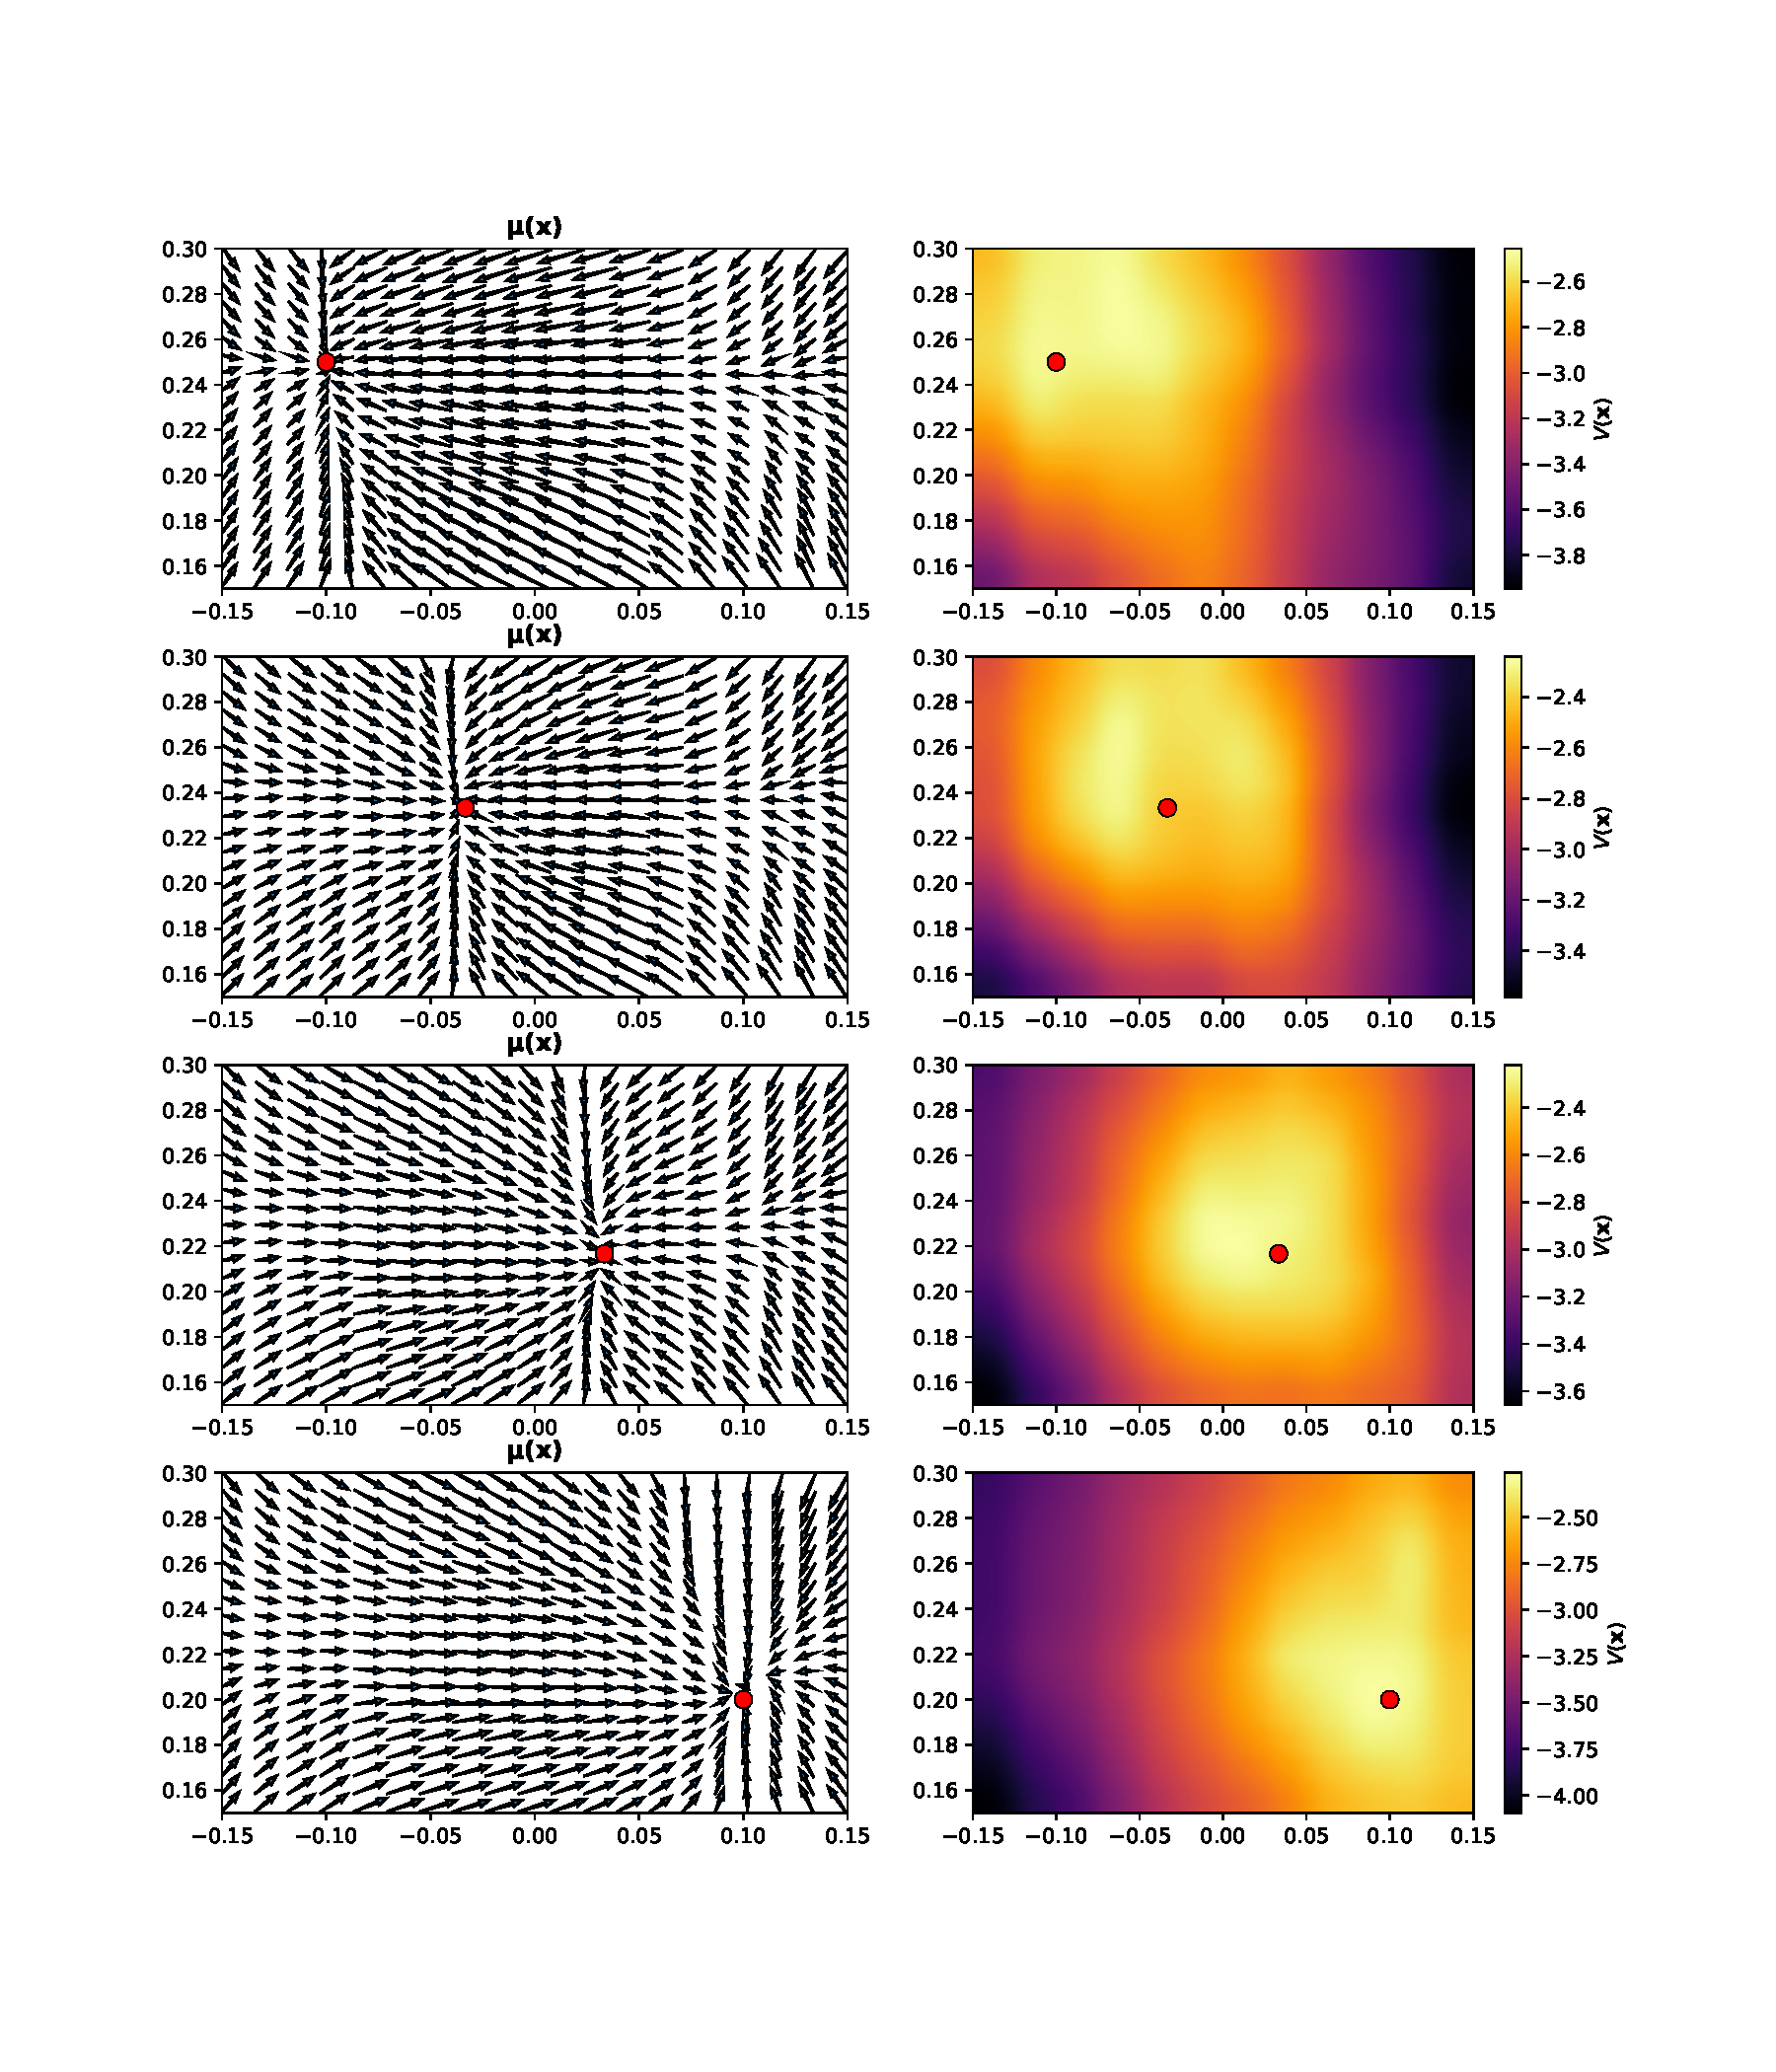
\includegraphics[width=\textwidth]{res/moving_goal_summary.pdf}

    \caption{Trained policy and value function for moving a simulated
    end-effector to randomly set goals. Vertical and horizontal axes are
    end-effector positions. Red dot is goal position. Left figure shows the
    learned policy $\mu$, right side shows the learned value function for
    different goal poses.}

    \label{fig:sim_moving_goal}
    
\end{figure}
